% linux-mcp approval-ticket finite state machine.
% Standalone; compile with: pdflatex linux-mcp-approval.tex
%
% States and transitions follow kernel-mcp: PENDING, APPROVED,
% CONSUMED, DENIED; EXPIRED is implicit (removal from ticket table).
\documentclass[tikz,border=4pt]{standalone}
\usepackage{tikz}
\usepackage{inconsolata}
\usetikzlibrary{positioning,calc,arrows.meta,shapes.geometric,fit,backgrounds}

\definecolor{edgeDark}{RGB}{70,70,70}
\definecolor{stFill}{RGB}{245,245,245}
\definecolor{allowFill}{RGB}{220,238,223}
\definecolor{denyFill}{RGB}{250,226,222}
\definecolor{deferFill}{RGB}{253,241,209}
\definecolor{consFill}{RGB}{220,232,250}

\begin{document}
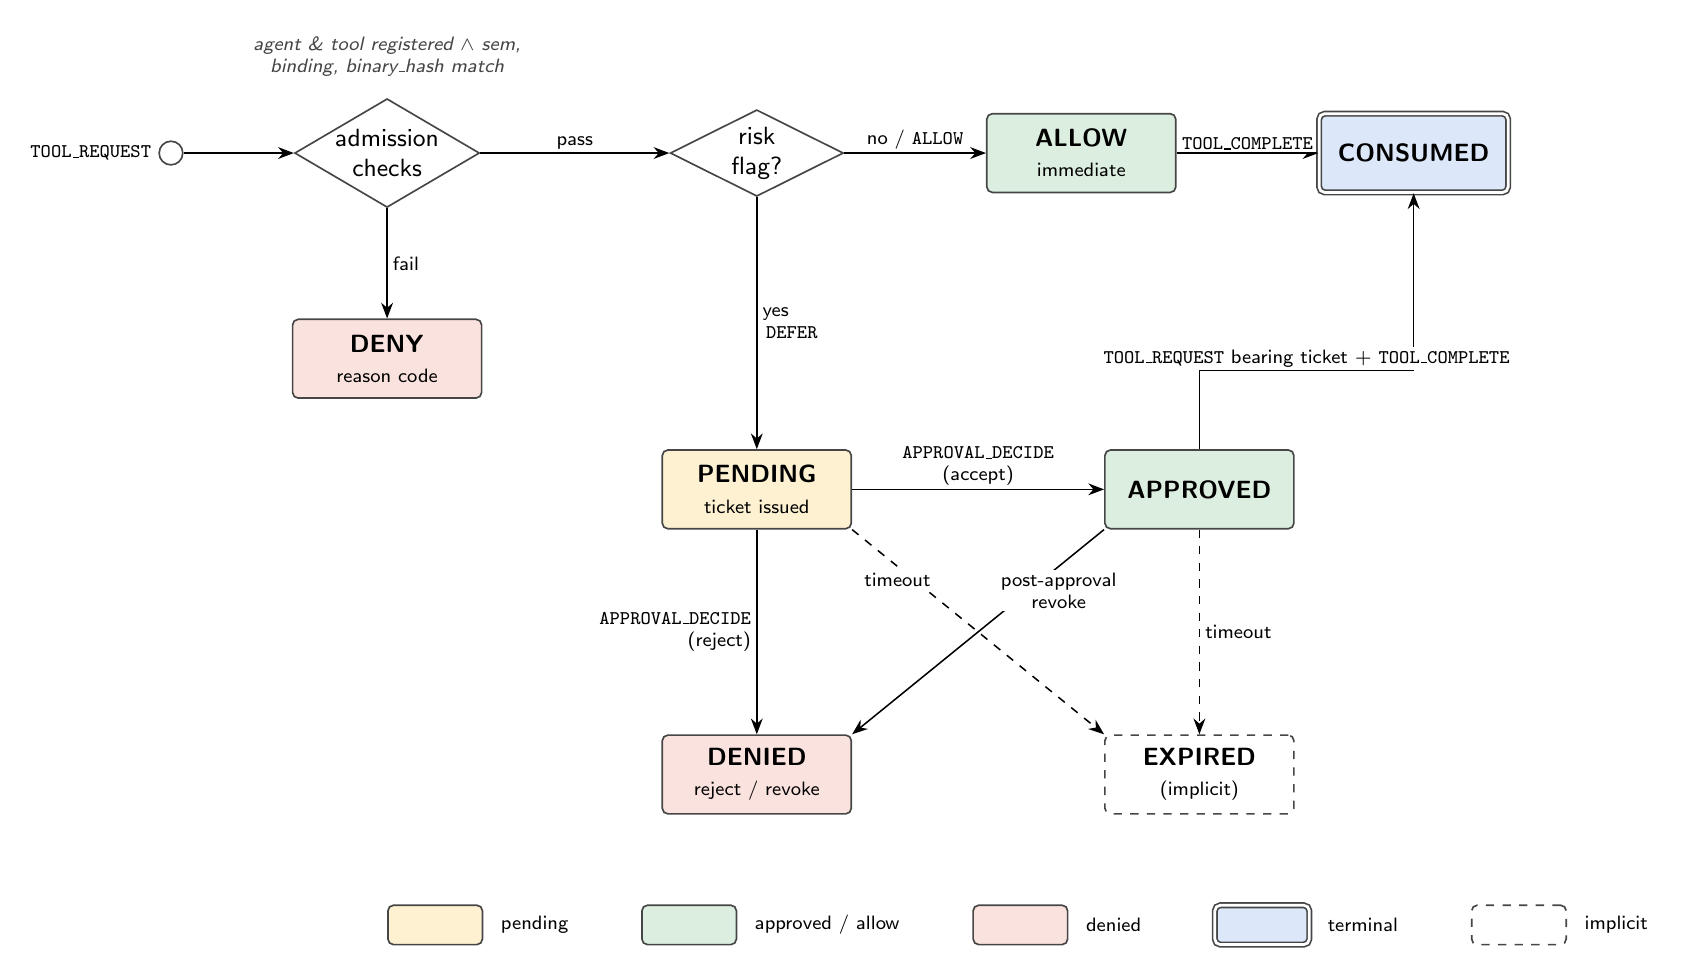
\begin{tikzpicture}[
  font=\small\sffamily,
  state/.style={draw=edgeDark,rounded corners=2pt,minimum width=24mm,
                minimum height=10mm,line width=0.6pt,align=center,fill=stFill},
  terminal/.style={state,double,double distance=1pt},
  decision/.style={draw=edgeDark,diamond,aspect=1.7,align=center,
                   line width=0.6pt,inner sep=0pt,minimum width=22mm,
                   minimum height=11mm,fill=white,font=\small\sffamily},
  entry/.style={draw=edgeDark,fill=white,circle,inner sep=1pt,
                minimum size=3mm,line width=0.6pt},
  tr/.style={-{Stealth[length=2mm]},line width=0.55pt},
  lbl/.style={font=\scriptsize\sffamily,fill=white,inner sep=1pt,align=center},
  guard/.style={font=\scriptsize\sffamily\itshape,text=edgeDark,align=center}
]

% ==========  ROW A: admission pipeline (top)  ==========
\node[entry] (start) at (0,0) {};
\node[lbl,left=0.5mm of start,fill=none] {\texttt{TOOL\_REQUEST}};

\node[decision,right=14mm of start] (adm) {admission\\checks};

\node[decision,right=24mm of adm] (risky) {risk\\flag?};

\node[state,fill=allowFill,right=18mm of risky] (allow)
  {\textbf{ALLOW}\\\scriptsize immediate};

\node[terminal,fill=consFill,right=18mm of allow] (consumed) {\textbf{CONSUMED}};

% Guard text above the admission diamond (doesn't collide with fail arrow below).
\node[guard,above=1.5mm of adm,text width=46mm]
  {agent \& tool registered\,\,$\wedge$\,\,sem, binding, binary\_hash match};

% ==========  ROW B: ticket FSM (middle, same y across)  ==========
\node[state,fill=deferFill,below=32mm of risky] (pending)
  {\textbf{PENDING}\\\scriptsize ticket issued};

\node[state,fill=allowFill,right=32mm of pending] (approved) {\textbf{APPROVED}};

% DENY (admission failure) sits under adm
\node[state,fill=denyFill,below=14mm of adm] (deny1)
  {\textbf{DENY}\\\scriptsize reason code};

% DENIED (ticket reject / revoke) sits under PENDING
\node[state,fill=denyFill,below=26mm of pending] (denied)
  {\textbf{DENIED}\\\scriptsize reject / revoke};

% EXPIRED (implicit) sits under APPROVED
\node[state,dashed,fill=white,draw=edgeDark,minimum width=24mm,
      minimum height=10mm,below=26mm of approved,align=center]
      (expired) {\textbf{EXPIRED}\\\scriptsize (implicit)};

% ==========  Transitions: admission pipeline  ==========
\draw[tr] (start) -- (adm.west);
\draw[tr] (adm.east) -- node[lbl,above]{pass} (risky.west);
\draw[tr] (adm.south) -- node[lbl,right=0.3mm]{fail} (deny1.north);

\draw[tr] (risky.east) -- node[lbl,above]{no / \texttt{ALLOW}} (allow.west);
\draw[tr] (risky.south) -- node[lbl,right=0.3mm,align=left]
           {yes\\\,\texttt{DEFER}} (pending.north);

\draw[tr] (allow.east) -- node[lbl,above]{\texttt{TOOL\_COMPLETE}} (consumed.west);

% ==========  Transitions: ticket FSM  ==========
\draw[tr] (pending) -- node[lbl,above,align=center]
  {\texttt{APPROVAL\_DECIDE}\\(accept)} (approved);

% APPROVED -> CONSUMED (routed up then right; label on the horizontal segment
% so it doesn't collide with APPROVAL_DECIDE(accept)).
\draw[tr] (approved.north) -- ++(0,10mm) -|
          node[lbl,pos=0.25,above,align=center]
          {\texttt{TOOL\_REQUEST} bearing ticket $+$ \texttt{TOOL\_COMPLETE}}
          (consumed.south);

% PENDING -> DENIED (reject; straight down, label on LEFT)
\draw[tr] (pending.south) -- node[lbl,left=0.3mm,align=right]
  {\texttt{APPROVAL\_DECIDE}\\(reject)} (denied.north);

% APPROVED -> EXPIRED (timeout, dashed, straight down, label on RIGHT)
\draw[tr,dashed] (approved.south) -- node[lbl,right=0.3mm]{timeout} (expired.north);

% APPROVED -> DENIED (post-approval revoke; diagonal, label placed near
% APPROVED end so it stays on the right-hand side and away from the
% PENDING->EXPIRED crossing label).
\draw[tr] (approved.south west) -- node[lbl,pos=0.18,below=0.4mm,align=center]
  {post-approval\\revoke} (denied.north east);

% PENDING -> EXPIRED (timeout, dashed, diagonal; label placed near
% PENDING end, on the left-hand side).
\draw[tr,dashed] (pending.south east) -- node[lbl,pos=0.18,below=0.4mm]
  {timeout} (expired.north west);

% ==========  Legend (single horizontal strip BELOW diagram)  ==========
% Anchor below DENIED/EXPIRED so it sits under the full FSM.
\begin{scope}[shift={($(denied.south -| adm)+(0,-14mm)$)}]
  \node[state,fill=deferFill,minimum width=12mm,minimum height=5mm,anchor=west] (lgA) at (0,0) {};
  \node[right=1mm of lgA,font=\scriptsize\sffamily,anchor=west] (lgAt) {pending};
  \node[state,fill=allowFill,minimum width=12mm,minimum height=5mm,right=8mm of lgAt,anchor=west] (lgB) {};
  \node[right=1mm of lgB,font=\scriptsize\sffamily,anchor=west] (lgBt) {approved / allow};
  \node[state,fill=denyFill,minimum width=12mm,minimum height=5mm,right=8mm of lgBt,anchor=west] (lgC) {};
  \node[right=1mm of lgC,font=\scriptsize\sffamily,anchor=west] (lgCt) {denied};
  \node[terminal,fill=consFill,minimum width=12mm,minimum height=5mm,right=8mm of lgCt,anchor=west] (lgD) {};
  \node[right=1mm of lgD,font=\scriptsize\sffamily,anchor=west] (lgDt) {terminal};
  \node[state,dashed,fill=white,minimum width=12mm,minimum height=5mm,right=8mm of lgDt,anchor=west] (lgE) {};
  \node[right=1mm of lgE,font=\scriptsize\sffamily,anchor=west] {implicit};
\end{scope}

% (call_log annotation removed by request.)

\end{tikzpicture}
\end{document}
